\documentclass{article}
\usepackage{graphicx} % Required for inserting images

\title{Final Labwork Advanced Programming for HPC}
\author{Ta Quang Hieu - M22ICT002}
\date{November 2023}

\begin{document}
	
	\maketitle
	
	\section{The problem}
	Final Labwork: Fine-art transformation
	
	• Implement Kuwahara filter, both with- and without- shared memory
	
	• Explain how you implement the labworks
	
	• Explain and measure speedup:
	\begin{itemize}
		\item • Without-shared memory vs CPU
		\item • With-shared memory vs without-shared memory
		\item • Other optimizations? Bank conflict? Coalesced access?
	\end{itemize}    
	
	% The general steps -> CPU -> gpu_no_sm-> gpu_sm
	
	\section{What is the Kuwahara filter}
	Kuwahara filter is a non-linear image filter used to reduce the notice while preserving the edges, this filter was introduced by Yoshinori Kuwahara in 1979.
	
	This filter works by calculate the average values of pixels in windows, then choose the window with the min standard variation. These are some advantages of Kuwahara filter:
	
	* Efficient to reduce noise
	
	* It preserves edges well, without blurring as much as other filters such as Gaussian filter.
	
	* Produces oil-painting effect
	
	However, Kuwahara filter will require a lot of computation. And that why we can take advantage of the parallel computing using GPU to implement this Kuwahara filter. In the next section, I will introduce the general logic steps of Kuwahara filter.
	
	\section{The general steps}
	
	The general steps of Kuwahara filter are listed below:
	
	\begin{itemize}
		\item We need a parameter $\omega$ as window size
		\item Then we need to convert the image from RGB to HSV (SCATTER)
		\item For each pixel $\Phi(i, j)$
		\begin{itemize}
			\item Define 4 windows $W_k$, $k \in [1..4]$ of size $(\omega + 1) \times (\omega + 1)$
			\begin{itemize}
				\item $W_1^x \in [i - \omega, i]$, $W_1^y \in [j - \omega, j]$
				\item $W_2^x \in [i, i + \omega]$, $W_2^y \in [j - \omega, j]$
				\item $W_3^x \in [i - \omega, i]$, $W_3^y \in [j, j + \omega]$
				\item $W_4^x \in [i, i + \omega]$, $W_4^y \in [j, j + \omega]$
			\end{itemize}
			\item Find $W_l$, $l \in [1..4]$ having lowest standard deviation of brightness.
			\item Use $V$ in HSV color space to calculate the standard deviation.
			\item Assign mean $(R, G, B)$ value of this window $|W_l|_\text{RGB}$ as new color (REDUCE, MAP) 
			\begin{itemize}
				\item $\Phi(i, j)_\text{RGB} = |W_l|_\text{RGB}$
			\end{itemize}
		\end{itemize}
	\end{itemize}
	
	For the following parts of implementing Kuwahara filter using CPU and GPU (with or without shared memory), I will still apply those general step. The next part will be how did I implement this filter using CPU.
	
	\section{Implementing Kuwahara filter using CPU}
	
	\subsection{Convert the image from RGB to HSV}
	
	After loaded the image, I will use a function to convert the image from RGB to HSV in order to use the V channel for calculating the windows standard deviation.
	
	This is the function that I used to turn the image from RGB to HSV.
	
	\begin{verbatim}
		from numba.typed import List
		
		#scale image [0..255] to [0..1]
		@cuda.jit(nopython=True)
		def scale(x):
		x = x/255
		return x
		
		#find max and min
		@cuda.jit(nopython=True)
		def min_and_max(red, green, blue, src):
		#find max
		if red > green and red > blue:
		max_c = (red, 0)
		elif green > red and green > blue:
		max_c = (green, 1)
		else:
		max_c = (blue, 2)
		
		#find min
		if red < green and red < blue:
		min_c = (red, 0)
		elif green < red and green < blue:
		min_c = (green, 1)
		else:
		min_c = (blue, 2)
		
		delta = max_c[0] - min_c[0]
		
		return (max_c, min_c, delta)
		
		@cuda.jit
		def rgb2hsv(src, dst):
		tidx = cuda.threadIdx.x + cuda.blockIdx.x * cuda.blockDim.x
		g = np.float32(((src[tidx, 0] + src[tidx, 1] + src[tidx, 2]) / 3))
		
		red = scale(np.float32(src[tidx, 0]))
		green = scale(np.float32(src[tidx, 1]))
		blue = scale(np.float32(src[tidx, 2]))
		
		# min_c, max_c, delta = min_and_max(red, green, blue, src)
		max_c, min_c, delta = min_and_max(red, green, blue, src)
		H = 0
		S = 0
		V = 0
		if delta == 0:
		H = 0
		elif max_c[1] == 0:
		H = 60*(((green-blue)/delta)%6)
		elif max_c[1] == 1:
		H = 60*(((blue-red)/delta)+2)
		else:
		H = 60*(((red-green)/delta)+4)
		
		if max_c[0] == 0:
		S = 0
		else:
		S = delta/max_c[0]
		
		V = max_c[0]
		
		dst[tidx, 0] = H
		dst[tidx, 1] = S
		dst[tidx, 2] = V
	\end{verbatim}
	
	The basic algorithm is taken from Gather-Scatter lecture for part 1 of the course Advanced programming for HPC in USTH. This function that turn the image from RGB to HSV by using GPU and for the convert to HSV step in the latter section will also be this function
	
	Figure ~\ref{fig:python} is the image that I used for this problem and Figure ~\ref{fig:hsv_python} show the result obtained after converted the image from RGB to HSV.
	
	\begin{figure}
		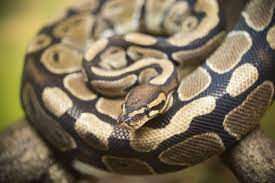
\includegraphics[width=\linewidth]{python.jpg}
		\caption{A python in RGB.}
		\label{fig:python}
	\end{figure}
	
	\begin{figure}
		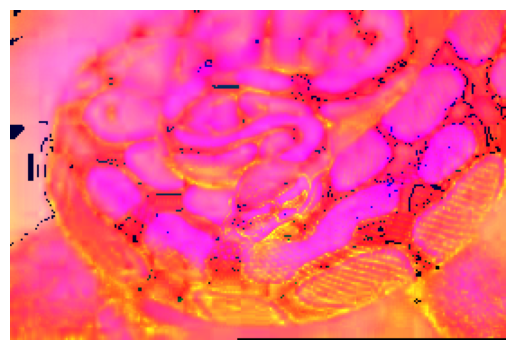
\includegraphics[width=\linewidth]{hsv_image.png}
		\caption{A python in HSV.}
		\label{fig:hsv_python}
	\end{figure}
	
	\subsection{Kuwahara filter}
	
	This is the function that I used to apply the Kuwahara filter for the image.
	
	\begin{verbatim}
		import numpy as np
		import cv2
		
		def kuwahara_filter(image, window_size):
		h, w, _ = image.shape
		# pad = window_size // 2
		output = np.zeros((h, w, 3))
		
		# pad the image
		image = cv2.copyMakeBorder(image, window_size, window_size, window_size, window_size, cv2.BORDER_REFLECT)
		
		# convert image to hsv
		# flatten the image into a 1D array of RGB
		imageWidth, imageHeight = image.shape[0], image.shape[1]
		pixel_count = imageWidth * imageHeight
		blockSize = 1024
		gridSize = int(pixel_count / blockSize)
		
		rgb_flat_1 = image.reshape(pixel_count, 3)
		
		start_time_gpu = time.time()
		devSrc = cuda.to_device(rgb_flat_1)
		devDst = cuda.device_array((pixel_count, 3), np.float32)
		rgb2hsv[gridSize, blockSize](devSrc, devDst)
		hostDst = devDst.copy_to_host()
		gpu_time = time.time() - start_time_gpu
		
		hsv_image = hostDst.reshape(imageWidth, imageHeight, 3)
		
		for i in range(window_size, h + window_size): # start at pad and end at h + pad (+pad is the start one)
		for j in range(window_size, w + window_size):
		windows = [
		image[i-window_size:i+1, j-window_size:j+1],
		image[i:i+window_size+1, j-window_size:j+1],
		image[i-window_size:i+1, j:j+window_size+1],
		image[i:i+window_size+1, j:j+window_size+1]
		]
		hsv_windows = [
		hsv_image[i-window_size:i+1, j-window_size:j+1, 2],
		hsv_image[i:i+window_size+1, j-window_size:j+1, 2],
		hsv_image[i-window_size:i+1, j:j+window_size+1, 2],
		hsv_image[i:i+window_size+1, j:j+window_size+1, 2]
		]
		
		# find the window with the lowest standard deviation of brightness
		std_devs = [np.std(win) for win in hsv_windows]
		best_win = windows[np.argmin(std_devs)]
		
		# assign the mean RGB value of this window to the output pixel
		output[i-window_size, j-window_size] = np.mean(np.mean(best_win, axis=0), axis=0)
		
		return output.astype('uint8')
	\end{verbatim}
	
	The function just followed the basic algorithms in the 3rd section, but before applying the filter to the image, Firstly I have to pad the image for the pixels that are near the border, because without padding the image, the windows for these pixels cannot be created.
	
	Figure ~\ref{fig:filter_image_cpu} is the result produced from the Kuwahara filter using CPU:
	
	\begin{figure}
		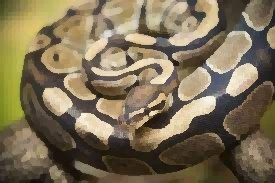
\includegraphics[width=\linewidth]{filtered_image_cpu.jpg}
		\caption{ Kuwahara filter using CPU}
		\label{fig:filter_image_cpu}
	\end{figure}
	
	\section{Implementing Kuwahara filter using GPU}
	
	\subsection{Without shared memory}
	
	I will still use the rgb2hsv function in the 4th section to convert the image from RGB to HSV and this is the function that I made for the Kuwahara filter.
	
	\begin{verbatim}
		import math
		
		@cuda.jit
		def kuwahara_filter_new(src, dst, v_arr, window_size):
		tidx = cuda.threadIdx.x + cuda.blockIdx.x * cuda.blockDim.x
		tidy = cuda.threadIdx.y + cuda.blockIdx.y * cuda.blockDim.y
		
		# test win1
		# hsv1 = hsv_image_part2[tidx-window_size:tidx, tidy-window_size:tidy, 2]
		sum_window1 = np.float32(0)
		for i in range(tidx-window_size, tidx):
		for j in range(tidy-window_size, tidy):
		sum_window1 += v_arr[i, j]
		mean_w1 = sum_window1/(window_size*window_size)
		
		sosd1 = np.float32(0)
		
		for i in range(tidx-window_size, tidx):
		for j in range(tidy-window_size, tidy):
		sosd1 += (v_arr[i, j] - mean_w1)*(v_arr[i, j] - mean_w1)
		
		std_dev1 = math.sqrt(sosd1/(window_size*window_size))
		# test win2
		# hsv2 = hsv_image_part2[tidx:tidx+window_size, tidy-window_size:tidy, 2]
		sum_window2 = np.float32(0)
		for i in range(tidx,tidx+window_size):
		for j in range(tidy-window_size,tidy):
		sum_window2 += v_arr[i, j]
		mean_w2 = sum_window2/(window_size*window_size)
		
		sosd2 = np.float32(0)
		
		for i in range(tidx,tidx+window_size):
		for j in range(tidy-window_size,tidy):
		sosd2 += (v_arr[i, j] - mean_w2)*(v_arr[i, j] - mean_w2)
		
		std_dev2 = math.sqrt(sosd2/(window_size*window_size))
		# test win3
		# hsv3 = hsv_image_part2[tidx-window_size:tidx, tidy:tidy+window_size, 2]
		sum_window3 = np.float32(0)
		for i in range(tidx-window_size,tidx):
		for j in range(tidy,tidy+window_size):
		sum_window3 += v_arr[i, j]
		mean_w3 = sum_window3/(window_size*window_size)
		
		sosd3 = np.float32(0)
		
		for i in range(tidx-window_size,tidx):
		for j in range(tidy,tidy+window_size):
		sosd3 += (v_arr[i, j] - mean_w3)*(v_arr[i, j] - mean_w3)
		
		std_dev3 = math.sqrt(sosd3/(window_size*window_size))
		# test win4
		# hsv4 = hsv_image_part2[tidx:tidx+window_size, tidy:tidy+window_size, 2]
		sum_window4 = np.float32(0)
		for i in range(tidx,tidx+window_size):
		for j in range(tidy,tidy+window_size):
		sum_window4 += v_arr[i, j]
		mean_w4 = sum_window4/(window_size*window_size)
		
		sosd4 = np.float32(0)
		
		for i in range(tidx,tidx+window_size):
		for j in range(tidy,tidy+window_size):
		sosd4 += (v_arr[i, j] - mean_w4)*(v_arr[i, j] - mean_w4)
		
		std_dev4 = math.sqrt(sosd4/(window_size*window_size))
		
		# till here, i have my 4 windows
		min_std_dev = min(std_dev1, std_dev2, std_dev3, std_dev4)
		
		R = np.float32(0)
		B = np.float32(0)
		G = np.float32(0)
		
		if std_dev1 == min_std_dev:
		for i in range(tidx-window_size, tidx):
		for j in range(tidy-window_size, tidy):
		R += src[i, j, 0]
		G += src[i, j, 1]
		B += src[i, j, 2]
		
		dst[tidx, tidy, 0] = np.uint8(R / (window_size*window_size))
		dst[tidx, tidy, 1] = np.uint8(G / (window_size*window_size))
		dst[tidx, tidy, 2] = np.uint8(B / (window_size*window_size))
		
		if std_dev2 == min_std_dev:
		for i in range(tidx,tidx+window_size):
		for j in range(tidy-window_size,tidy):
		R += src[i, j, 0]
		G += src[i, j, 1]
		B += src[i, j, 2]
		
		dst[tidx, tidy, 0] = np.uint8(R / (window_size*window_size))
		dst[tidx, tidy, 1] = np.uint8(G / (window_size*window_size))
		dst[tidx, tidy, 2] = np.uint8(B / (window_size*window_size))
		
		if std_dev3 == min_std_dev:
		for i in range(tidx-window_size,tidx):
		for j in range(tidy,tidy+window_size):
		R += src[i, j, 0]
		G += src[i, j, 1]
		B += src[i, j, 2]
		
		dst[tidx, tidy, 0] = np.uint8(R / (window_size*window_size))
		dst[tidx, tidy, 1] = np.uint8(G / (window_size*window_size))
		dst[tidx, tidy, 2] = np.uint8(B / (window_size*window_size))
		
		if std_dev4 == min_std_dev:
		for i in range(tidx,tidx+window_size):
		for j in range(tidy,tidy+window_size):
		R += src[i, j, 0]
		G += src[i, j, 1]
		B += src[i, j, 2]
		
		# dst[tidx, tidy, 0] = R / (window_size*window_size)
		# dst[tidx, tidy, 1] = G / (window_size*window_size)
		# dst[tidx, tidy, 2] = B / (window_size*window_size)
		
		dst[tidx, tidy, 0] = np.uint8(R / (window_size*window_size))
		dst[tidx, tidy, 1] = np.uint8(G / (window_size*window_size))
		dst[tidx, tidy, 2] = np.uint8(B / (window_size*window_size))
		
		# Flatten the image into a 1D array of RGB
		imageWidth, imageHeight  = rgb_image_new.shape[0], rgb_image_new.shape[1]
		pixel_count = imageWidth * imageHeight
		
		blockDim = (16, 16)
		gridDim = ((imageWidth // blockDim[0]) + 1, (imageHeight // blockDim[1]) + 1)
		
		# v_arr = hsv_image_part2[tidx-window_size:tidx, tidy-window_size:tidy, 2]
		
		v_arr = hsv_image_part2[:, :, 2]
		v_arr = np.ascontiguousarray(v_arr)
		
		devSrc = cuda.to_device(rgb_image_new)
		devDst = cuda.device_array((imageWidth, imageHeight, 3), np.uint8)
		cuda_v_arr = cuda.to_device(v_arr)
		# v_chanel = cuda.to_device(v_arr)
		# grayscale[gridSize, blockSize](devSrc, devDst)
		start_time_gpu = time.time()
		kuwahara_filter_new[gridDim, blockDim](devSrc, devDst, cuda_v_arr, 5)
		hostDst = devDst.copy_to_host()
		gpu_time = time.time() - start_time_gpu
		
		new_image_kuwahara = hostDst.reshape(imageWidth, imageHeight, 3)
		
		plt.imshow(new_image_kuwahara)
		plt.axis('off')
		plt.show()
	\end{verbatim}
	
	The input for this function is the original image in RGB, an array to store the result, the v channel of the image after being converted to HSV in order to be used to calculate the standard deviation, and finally the window size. I struggled with this for a while since I cannot use the regular operation as I used to use with the CPU like creating multiple lists inside a list or using some numpy function. Below is the first version before I realized that I would need to separate it into several individual lists and loops which made the function become really long or it is just because that I did not know the better way to do it. 
	
	\begin{verbatim}
		# the src will be my initial rgb image and the hsv will be use for the shared mem later
		@cuda.jit
		def kuwahara_filter_new(src, dst, window_size):
		tidx = cuda.threadIdx.x + cuda.blockIdx.x * cuda.blockDim.x
		tidy = cuda.threadIdx.y + cuda.blockIdx.y * cuda.blockDim.y
		
		# H = scale(np.float32(src[tidx, 0]))
		# S = scale(np.float32(src[tidx, 1]))
		# V = scale(np.float32(src[tidx, 2]))
		
		# =============================================
		# for i in range(window_size, imageHeight + window_size): # start at pad and end at h + pad (+pad is the start one)
		#     for j in range(window_size, imageWidth + window_size):
		windows = [
		src[tidx-window_size:tidx+1, tidy-window_size:tidy+1],
		src[tidx:tidx+window_size+1, tidy-window_size:tidy+1],
		src[tidx-window_size:tidx+1, tidy:tidy+window_size+1],
		src[tidx:tidx+window_size+1, tidy:tidy+window_size+1]
		]
		hsv_windows = [
		hsv_image_part2[tidx-window_size:tidx+1, tidy-window_size:tidy+1, 2],
		hsv_image_part2[tidx:tidx+window_size+1, tidy-window_size:tidy+1, 2],
		hsv_image_part2[tidx-window_size:tidx+1, tidy:tidy+window_size+1, 2],
		hsv_image_part2[tidx:tidx+window_size+1, tidy:tidy+window_size+1, 2]
		]
		
		# # find the window with the lowest standard deviation of brightness
		# std_devs = [np.std(win) for win in hsv_windows]
		# best_win = windows[np.argmin(std_devs)]
		
		# find the window with the lowest standard deviation of brightness
		std_devs = []
		for win in hsv_windows:
		mean = win.sum() / win.size
		std_dev = np.sqrt(((win - mean)**2).sum() / win.size)
		std_devs.append(std_dev)
		best_win = windows[np.argmin(std_devs)]
		
		# assign the mean RGB value of this window to the output pixel
		# dst[tidx-window_size, tidy-window_size] = np.mean(np.mean(best_win, axis=0), axis=0)
		mean_rgb = best_win.sum(axis=(0, 1)) / (best_win.shape[0] * best_win.shape[1])
		dst[tidx-window_size, tidy-window_size] = mean_rgb
		# =============================================
		
		# dst[tidx, 0] = H
		# dst[tidx, 1] = S
		# dst[tidx, 2] = V
		# dst[tidx, tidy, 0] = dst[tidx, tidy, 1] = dst[tidx, tidy, 2] = g
	\end{verbatim}
	
	As you can see it is much shorter but it just doesn't work=))
	
	Figure ~\ref{fig:filter_image_gpu} is the result produced from the Kuwahara filter using GPU:
	
	\begin{figure}
		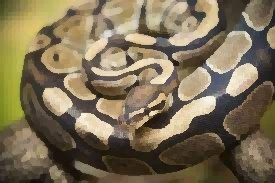
\includegraphics[width=\linewidth]{filtered_image_gpu.jpg}
		\caption{ Kuwahara filter using GPU}
		\label{fig:filter_image_gpu}
	\end{figure}
	
	\subsection{With shared memory}
	
	For the implementation using shared memory, I decided to put the v channel of the HSV image into the shared memory because we will have to access it frequently. I just added the following code to the filter.
	
	\begin{verbatim}
		shared = cuda.shared.array((183, 275), numba.uint8)
		shared = v_chanel
		cuda.syncthreads()
	\end{verbatim}
	
	I had settled the Constance value for the dimension here since I tried to send the shape0 and shape1 parameters but I don't know how to do it after several attempts so I will just set them like that. I used the command cuda.syncthread() to ensure that all the threads would finish copying the vchanel before coming to the next step. And of course the image result will still be the same as using CPU or GPU without shared memory show I will not show it again.
	
	\section{Comparition}
	
	The Table~\ref{tab:running_3_method} shows the running time of using CPU, GPU-with and without shared memory with a window size is 5. The result is the average obtained by running those methods 5 times.
	
	\begin{tabular}{|c|c|c|c|}
		\hline
		Window Size & CPU & GPU (Without Shared Memory) & GPU (With Shared Memory) \\ \hline
		5 & 9.7689 s & 1.7395 s & 0.00157 s \\ \hline
		\label{tab:running_3_method}
	\end{tabular}
	
	You can easily see that the running time of the CPU is longer than the GPU without shared memory and GPU with shared memory and the GPU that use shared memory run much faster than the previous method since it doesn't need to come back to find the global variable. Using shared memory also helped me, initially when implementing the GPU without shared memory it was really hard and always gave me the error that I was using too much memory for the constant global variables, and using shared memory helped me to get rid of that.
	
	The Table~\ref{tab:running_GPU_SM} shows the running time of using GPU with shared memory with multiple window sizes.
	
	\begin{tabular}{|c|c|c|c|c|}
		\hline
		Window Size & 3 & 5 & 7 & 9 \\ \hline
		GPU (With Shared Memory) & 0.00569 s & 0.00115 s & 0.00164 s & 0.00228 s  \\ \hline
		\label{tab:running_3_method}
	\end{tabular}
	
	Actually, the result is like below where the first 2 value are both the window size of 3 but somehow the second time take longer, but in general we can see that the running time is increase as the window size increase since we need to perform more computation as the window size increase:
	\begin{verbatim}
		[0.0010039806365966797,
		0.005692243576049805,
		0.0011553764343261719,
		0.0016481876373291016,
		0.002286672592163086]
	\end{verbatim}
	
\end{document}
